% Created by tikzDevice version 0.12.3.1 on 2023-06-22 13:18:05
% !TEX encoding = UTF-8 Unicode
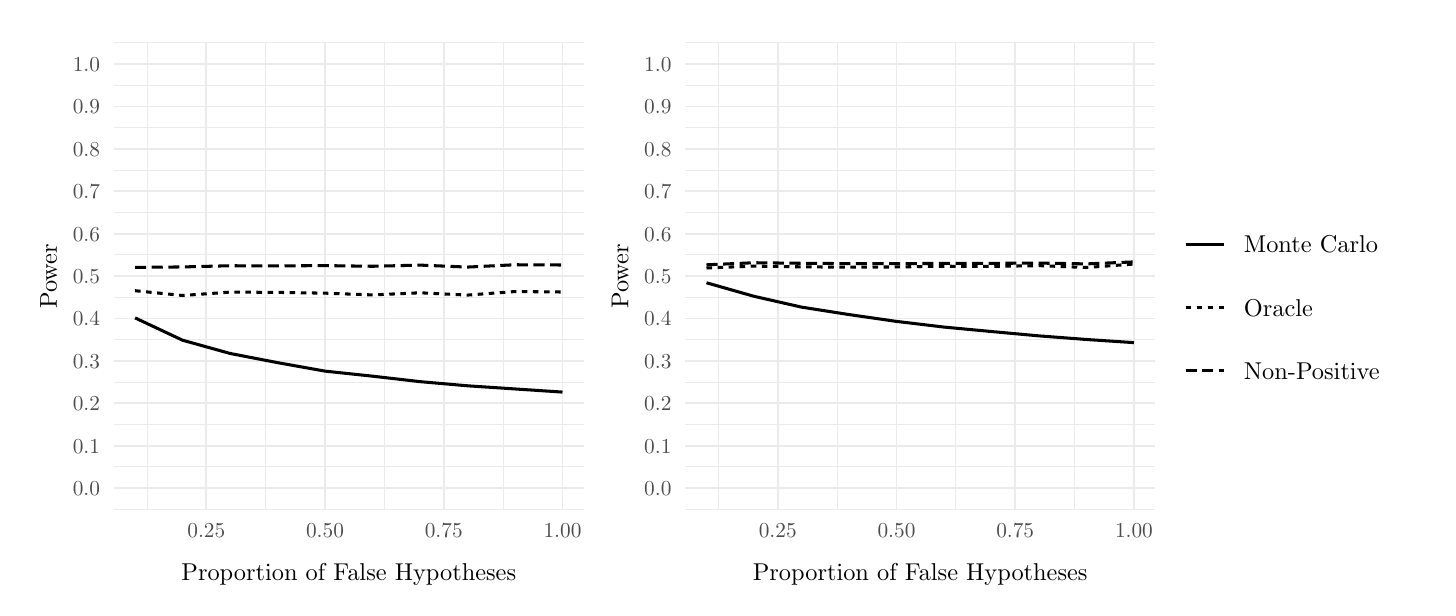
\begin{tikzpicture}[x=1pt,y=1pt]
\definecolor{fillColor}{RGB}{255,255,255}
\path[use as bounding box,fill=fillColor,fill opacity=0.00] (0,0) rectangle (505.89,202.36);
\begin{scope}
\path[clip] ( 31.08, 28.32) rectangle (200.99,196.86);
\definecolor{drawColor}{gray}{0.92}

\path[draw=drawColor,line width= 0.3pt,line join=round] ( 31.08, 28.32) --
	(200.99, 28.32);

\path[draw=drawColor,line width= 0.3pt,line join=round] ( 31.08, 43.64) --
	(200.99, 43.64);

\path[draw=drawColor,line width= 0.3pt,line join=round] ( 31.08, 58.96) --
	(200.99, 58.96);

\path[draw=drawColor,line width= 0.3pt,line join=round] ( 31.08, 74.28) --
	(200.99, 74.28);

\path[draw=drawColor,line width= 0.3pt,line join=round] ( 31.08, 89.60) --
	(200.99, 89.60);

\path[draw=drawColor,line width= 0.3pt,line join=round] ( 31.08,104.93) --
	(200.99,104.93);

\path[draw=drawColor,line width= 0.3pt,line join=round] ( 31.08,120.25) --
	(200.99,120.25);

\path[draw=drawColor,line width= 0.3pt,line join=round] ( 31.08,135.57) --
	(200.99,135.57);

\path[draw=drawColor,line width= 0.3pt,line join=round] ( 31.08,150.89) --
	(200.99,150.89);

\path[draw=drawColor,line width= 0.3pt,line join=round] ( 31.08,166.21) --
	(200.99,166.21);

\path[draw=drawColor,line width= 0.3pt,line join=round] ( 31.08,181.53) --
	(200.99,181.53);

\path[draw=drawColor,line width= 0.3pt,line join=round] ( 31.08,196.86) --
	(200.99,196.86);

\path[draw=drawColor,line width= 0.3pt,line join=round] ( 43.10, 28.32) --
	( 43.10,196.86);

\path[draw=drawColor,line width= 0.3pt,line join=round] ( 86.00, 28.32) --
	( 86.00,196.86);

\path[draw=drawColor,line width= 0.3pt,line join=round] (128.91, 28.32) --
	(128.91,196.86);

\path[draw=drawColor,line width= 0.3pt,line join=round] (171.81, 28.32) --
	(171.81,196.86);

\path[draw=drawColor,line width= 0.6pt,line join=round] ( 31.08, 35.98) --
	(200.99, 35.98);

\path[draw=drawColor,line width= 0.6pt,line join=round] ( 31.08, 51.30) --
	(200.99, 51.30);

\path[draw=drawColor,line width= 0.6pt,line join=round] ( 31.08, 66.62) --
	(200.99, 66.62);

\path[draw=drawColor,line width= 0.6pt,line join=round] ( 31.08, 81.94) --
	(200.99, 81.94);

\path[draw=drawColor,line width= 0.6pt,line join=round] ( 31.08, 97.27) --
	(200.99, 97.27);

\path[draw=drawColor,line width= 0.6pt,line join=round] ( 31.08,112.59) --
	(200.99,112.59);

\path[draw=drawColor,line width= 0.6pt,line join=round] ( 31.08,127.91) --
	(200.99,127.91);

\path[draw=drawColor,line width= 0.6pt,line join=round] ( 31.08,143.23) --
	(200.99,143.23);

\path[draw=drawColor,line width= 0.6pt,line join=round] ( 31.08,158.55) --
	(200.99,158.55);

\path[draw=drawColor,line width= 0.6pt,line join=round] ( 31.08,173.87) --
	(200.99,173.87);

\path[draw=drawColor,line width= 0.6pt,line join=round] ( 31.08,189.20) --
	(200.99,189.20);

\path[draw=drawColor,line width= 0.6pt,line join=round] ( 64.55, 28.32) --
	( 64.55,196.86);

\path[draw=drawColor,line width= 0.6pt,line join=round] (107.45, 28.32) --
	(107.45,196.86);

\path[draw=drawColor,line width= 0.6pt,line join=round] (150.36, 28.32) --
	(150.36,196.86);

\path[draw=drawColor,line width= 0.6pt,line join=round] (193.26, 28.32) --
	(193.26,196.86);
\definecolor{drawColor}{RGB}{0,0,0}

\path[draw=drawColor,line width= 1.1pt,line join=round] ( 38.81, 97.49) --
	( 55.97, 89.42) --
	( 73.13, 84.64) --
	( 90.29, 81.32) --
	(107.45, 78.25) --
	(124.62, 76.43) --
	(141.78, 74.45) --
	(158.94, 72.95) --
	(176.10, 71.81) --
	(193.26, 70.68);

\path[draw=drawColor,line width= 1.1pt,dash pattern=on 2pt off 2pt ,line join=round] ( 38.81,107.31) --
	( 55.97,105.58) --
	( 73.13,106.81) --
	( 90.29,106.70) --
	(107.45,106.42) --
	(124.62,105.79) --
	(141.78,106.56) --
	(158.94,105.73) --
	(176.10,107.01) --
	(193.26,106.84);

\path[draw=drawColor,line width= 1.1pt,dash pattern=on 4pt off 2pt ,line join=round] ( 38.81,115.74) --
	( 55.97,115.90) --
	( 73.13,116.33) --
	( 90.29,116.27) --
	(107.45,116.38) --
	(124.62,116.14) --
	(141.78,116.56) --
	(158.94,115.85) --
	(176.10,116.69) --
	(193.26,116.60);
\end{scope}
\begin{scope}
\path[clip] (  0.00,  0.00) rectangle (505.89,202.36);
\definecolor{drawColor}{gray}{0.30}

\node[text=drawColor,anchor=base east,inner sep=0pt, outer sep=0pt, scale=  0.77] at ( 26.13, 33.33) {0.0};

\node[text=drawColor,anchor=base east,inner sep=0pt, outer sep=0pt, scale=  0.77] at ( 26.13, 48.65) {0.1};

\node[text=drawColor,anchor=base east,inner sep=0pt, outer sep=0pt, scale=  0.77] at ( 26.13, 63.97) {0.2};

\node[text=drawColor,anchor=base east,inner sep=0pt, outer sep=0pt, scale=  0.77] at ( 26.13, 79.29) {0.3};

\node[text=drawColor,anchor=base east,inner sep=0pt, outer sep=0pt, scale=  0.77] at ( 26.13, 94.61) {0.4};

\node[text=drawColor,anchor=base east,inner sep=0pt, outer sep=0pt, scale=  0.77] at ( 26.13,109.94) {0.5};

\node[text=drawColor,anchor=base east,inner sep=0pt, outer sep=0pt, scale=  0.77] at ( 26.13,125.26) {0.6};

\node[text=drawColor,anchor=base east,inner sep=0pt, outer sep=0pt, scale=  0.77] at ( 26.13,140.58) {0.7};

\node[text=drawColor,anchor=base east,inner sep=0pt, outer sep=0pt, scale=  0.77] at ( 26.13,155.90) {0.8};

\node[text=drawColor,anchor=base east,inner sep=0pt, outer sep=0pt, scale=  0.77] at ( 26.13,171.22) {0.9};

\node[text=drawColor,anchor=base east,inner sep=0pt, outer sep=0pt, scale=  0.77] at ( 26.13,186.54) {1.0};
\end{scope}
\begin{scope}
\path[clip] (  0.00,  0.00) rectangle (505.89,202.36);
\definecolor{drawColor}{gray}{0.30}

\node[text=drawColor,anchor=base,inner sep=0pt, outer sep=0pt, scale=  0.77] at ( 64.55, 18.06) {0.25};

\node[text=drawColor,anchor=base,inner sep=0pt, outer sep=0pt, scale=  0.77] at (107.45, 18.06) {0.50};

\node[text=drawColor,anchor=base,inner sep=0pt, outer sep=0pt, scale=  0.77] at (150.36, 18.06) {0.75};

\node[text=drawColor,anchor=base,inner sep=0pt, outer sep=0pt, scale=  0.77] at (193.26, 18.06) {1.00};
\end{scope}
\begin{scope}
\path[clip] (  0.00,  0.00) rectangle (505.89,202.36);
\definecolor{drawColor}{RGB}{0,0,0}

\node[text=drawColor,anchor=base,inner sep=0pt, outer sep=0pt, scale=  0.88] at (116.04,  2.52) {Proportion of False Hypotheses};
\end{scope}
\begin{scope}
\path[clip] (  0.00,  0.00) rectangle (505.89,202.36);
\definecolor{drawColor}{RGB}{0,0,0}

\node[text=drawColor,rotate= 90.00,anchor=base,inner sep=0pt, outer sep=0pt, scale=  0.88] at ( 10.57,112.59) {Power};
\end{scope}
\begin{scope}
\path[clip] (237.57, 28.32) rectangle (407.47,196.86);
\definecolor{drawColor}{gray}{0.92}

\path[draw=drawColor,line width= 0.3pt,line join=round] (237.57, 28.32) --
	(407.47, 28.32);

\path[draw=drawColor,line width= 0.3pt,line join=round] (237.57, 43.64) --
	(407.47, 43.64);

\path[draw=drawColor,line width= 0.3pt,line join=round] (237.57, 58.96) --
	(407.47, 58.96);

\path[draw=drawColor,line width= 0.3pt,line join=round] (237.57, 74.28) --
	(407.47, 74.28);

\path[draw=drawColor,line width= 0.3pt,line join=round] (237.57, 89.60) --
	(407.47, 89.60);

\path[draw=drawColor,line width= 0.3pt,line join=round] (237.57,104.93) --
	(407.47,104.93);

\path[draw=drawColor,line width= 0.3pt,line join=round] (237.57,120.25) --
	(407.47,120.25);

\path[draw=drawColor,line width= 0.3pt,line join=round] (237.57,135.57) --
	(407.47,135.57);

\path[draw=drawColor,line width= 0.3pt,line join=round] (237.57,150.89) --
	(407.47,150.89);

\path[draw=drawColor,line width= 0.3pt,line join=round] (237.57,166.21) --
	(407.47,166.21);

\path[draw=drawColor,line width= 0.3pt,line join=round] (237.57,181.53) --
	(407.47,181.53);

\path[draw=drawColor,line width= 0.3pt,line join=round] (237.57,196.86) --
	(407.47,196.86);

\path[draw=drawColor,line width= 0.3pt,line join=round] (249.58, 28.32) --
	(249.58,196.86);

\path[draw=drawColor,line width= 0.3pt,line join=round] (292.49, 28.32) --
	(292.49,196.86);

\path[draw=drawColor,line width= 0.3pt,line join=round] (335.39, 28.32) --
	(335.39,196.86);

\path[draw=drawColor,line width= 0.3pt,line join=round] (378.30, 28.32) --
	(378.30,196.86);

\path[draw=drawColor,line width= 0.6pt,line join=round] (237.57, 35.98) --
	(407.47, 35.98);

\path[draw=drawColor,line width= 0.6pt,line join=round] (237.57, 51.30) --
	(407.47, 51.30);

\path[draw=drawColor,line width= 0.6pt,line join=round] (237.57, 66.62) --
	(407.47, 66.62);

\path[draw=drawColor,line width= 0.6pt,line join=round] (237.57, 81.94) --
	(407.47, 81.94);

\path[draw=drawColor,line width= 0.6pt,line join=round] (237.57, 97.27) --
	(407.47, 97.27);

\path[draw=drawColor,line width= 0.6pt,line join=round] (237.57,112.59) --
	(407.47,112.59);

\path[draw=drawColor,line width= 0.6pt,line join=round] (237.57,127.91) --
	(407.47,127.91);

\path[draw=drawColor,line width= 0.6pt,line join=round] (237.57,143.23) --
	(407.47,143.23);

\path[draw=drawColor,line width= 0.6pt,line join=round] (237.57,158.55) --
	(407.47,158.55);

\path[draw=drawColor,line width= 0.6pt,line join=round] (237.57,173.87) --
	(407.47,173.87);

\path[draw=drawColor,line width= 0.6pt,line join=round] (237.57,189.20) --
	(407.47,189.20);

\path[draw=drawColor,line width= 0.6pt,line join=round] (271.04, 28.32) --
	(271.04,196.86);

\path[draw=drawColor,line width= 0.6pt,line join=round] (313.94, 28.32) --
	(313.94,196.86);

\path[draw=drawColor,line width= 0.6pt,line join=round] (356.84, 28.32) --
	(356.84,196.86);

\path[draw=drawColor,line width= 0.6pt,line join=round] (399.75, 28.32) --
	(399.75,196.86);
\definecolor{drawColor}{RGB}{0,0,0}

\path[draw=drawColor,line width= 1.1pt,line join=round] (245.29,110.18) --
	(262.45,105.29) --
	(279.62,101.38) --
	(296.78, 98.69) --
	(313.94, 96.22) --
	(331.10, 94.17) --
	(348.26, 92.56) --
	(365.43, 90.99) --
	(382.59, 89.69) --
	(399.75, 88.54);

\path[draw=drawColor,line width= 1.1pt,dash pattern=on 2pt off 2pt ,line join=round] (245.29,115.52) --
	(262.45,116.20) --
	(279.62,115.94) --
	(296.78,115.81) --
	(313.94,115.90) --
	(331.10,116.15) --
	(348.26,116.09) --
	(365.43,116.37) --
	(382.59,115.69) --
	(399.75,116.95);

\path[draw=drawColor,line width= 1.1pt,dash pattern=on 4pt off 2pt ,line join=round] (245.29,116.67) --
	(262.45,117.42) --
	(279.62,117.22) --
	(296.78,117.09) --
	(313.94,117.09) --
	(331.10,117.18) --
	(348.26,117.20) --
	(365.43,117.29) --
	(382.59,117.00) --
	(399.75,117.72);
\end{scope}
\begin{scope}
\path[clip] (  0.00,  0.00) rectangle (505.89,202.36);
\definecolor{drawColor}{gray}{0.30}

\node[text=drawColor,anchor=base east,inner sep=0pt, outer sep=0pt, scale=  0.77] at (232.62, 33.33) {0.0};

\node[text=drawColor,anchor=base east,inner sep=0pt, outer sep=0pt, scale=  0.77] at (232.62, 48.65) {0.1};

\node[text=drawColor,anchor=base east,inner sep=0pt, outer sep=0pt, scale=  0.77] at (232.62, 63.97) {0.2};

\node[text=drawColor,anchor=base east,inner sep=0pt, outer sep=0pt, scale=  0.77] at (232.62, 79.29) {0.3};

\node[text=drawColor,anchor=base east,inner sep=0pt, outer sep=0pt, scale=  0.77] at (232.62, 94.61) {0.4};

\node[text=drawColor,anchor=base east,inner sep=0pt, outer sep=0pt, scale=  0.77] at (232.62,109.94) {0.5};

\node[text=drawColor,anchor=base east,inner sep=0pt, outer sep=0pt, scale=  0.77] at (232.62,125.26) {0.6};

\node[text=drawColor,anchor=base east,inner sep=0pt, outer sep=0pt, scale=  0.77] at (232.62,140.58) {0.7};

\node[text=drawColor,anchor=base east,inner sep=0pt, outer sep=0pt, scale=  0.77] at (232.62,155.90) {0.8};

\node[text=drawColor,anchor=base east,inner sep=0pt, outer sep=0pt, scale=  0.77] at (232.62,171.22) {0.9};

\node[text=drawColor,anchor=base east,inner sep=0pt, outer sep=0pt, scale=  0.77] at (232.62,186.54) {1.0};
\end{scope}
\begin{scope}
\path[clip] (  0.00,  0.00) rectangle (505.89,202.36);
\definecolor{drawColor}{gray}{0.30}

\node[text=drawColor,anchor=base,inner sep=0pt, outer sep=0pt, scale=  0.77] at (271.04, 18.06) {0.25};

\node[text=drawColor,anchor=base,inner sep=0pt, outer sep=0pt, scale=  0.77] at (313.94, 18.06) {0.50};

\node[text=drawColor,anchor=base,inner sep=0pt, outer sep=0pt, scale=  0.77] at (356.84, 18.06) {0.75};

\node[text=drawColor,anchor=base,inner sep=0pt, outer sep=0pt, scale=  0.77] at (399.75, 18.06) {1.00};
\end{scope}
\begin{scope}
\path[clip] (  0.00,  0.00) rectangle (505.89,202.36);
\definecolor{drawColor}{RGB}{0,0,0}

\node[text=drawColor,anchor=base,inner sep=0pt, outer sep=0pt, scale=  0.88] at (322.52,  2.52) {Proportion of False Hypotheses};
\end{scope}
\begin{scope}
\path[clip] (  0.00,  0.00) rectangle (505.89,202.36);
\definecolor{drawColor}{RGB}{0,0,0}

\node[text=drawColor,rotate= 90.00,anchor=base,inner sep=0pt, outer sep=0pt, scale=  0.88] at (217.05,112.59) {Power};
\end{scope}
\begin{scope}
\path[clip] (  0.00,  0.00) rectangle (505.89,202.36);
\definecolor{drawColor}{RGB}{0,0,0}

\path[draw=drawColor,line width= 1.1pt,line join=round] (418.39,124.02) -- (432.27,124.02);
\end{scope}
\begin{scope}
\path[clip] (  0.00,  0.00) rectangle (505.89,202.36);
\definecolor{drawColor}{RGB}{0,0,0}

\path[draw=drawColor,line width= 1.1pt,line join=round] (418.39,124.02) -- (432.27,124.02);
\end{scope}
\begin{scope}
\path[clip] (  0.00,  0.00) rectangle (505.89,202.36);
\definecolor{drawColor}{RGB}{0,0,0}

\path[draw=drawColor,line width= 1.1pt,line join=round] (418.39,124.02) -- (432.27,124.02);
\end{scope}
\begin{scope}
\path[clip] (  0.00,  0.00) rectangle (505.89,202.36);
\definecolor{drawColor}{RGB}{0,0,0}

\path[draw=drawColor,line width= 1.1pt,dash pattern=on 2pt off 2pt ,line join=round] (418.39,101.18) -- (432.27,101.18);
\end{scope}
\begin{scope}
\path[clip] (  0.00,  0.00) rectangle (505.89,202.36);
\definecolor{drawColor}{RGB}{0,0,0}

\path[draw=drawColor,line width= 1.1pt,dash pattern=on 2pt off 2pt ,line join=round] (418.39,101.18) -- (432.27,101.18);
\end{scope}
\begin{scope}
\path[clip] (  0.00,  0.00) rectangle (505.89,202.36);
\definecolor{drawColor}{RGB}{0,0,0}

\path[draw=drawColor,line width= 1.1pt,dash pattern=on 2pt off 2pt ,line join=round] (418.39,101.18) -- (432.27,101.18);
\end{scope}
\begin{scope}
\path[clip] (  0.00,  0.00) rectangle (505.89,202.36);
\definecolor{drawColor}{RGB}{0,0,0}

\path[draw=drawColor,line width= 1.1pt,dash pattern=on 4pt off 2pt ,line join=round] (418.39, 78.33) -- (432.27, 78.33);
\end{scope}
\begin{scope}
\path[clip] (  0.00,  0.00) rectangle (505.89,202.36);
\definecolor{drawColor}{RGB}{0,0,0}

\path[draw=drawColor,line width= 1.1pt,dash pattern=on 4pt off 2pt ,line join=round] (418.39, 78.33) -- (432.27, 78.33);
\end{scope}
\begin{scope}
\path[clip] (  0.00,  0.00) rectangle (505.89,202.36);
\definecolor{drawColor}{RGB}{0,0,0}

\path[draw=drawColor,line width= 1.1pt,dash pattern=on 4pt off 2pt ,line join=round] (418.39, 78.33) -- (432.27, 78.33);
\end{scope}
\begin{scope}
\path[clip] (  0.00,  0.00) rectangle (505.89,202.36);
\definecolor{drawColor}{RGB}{0,0,0}

\node[text=drawColor,anchor=base west,inner sep=0pt, outer sep=0pt, scale=  0.88] at (439.51,120.99) {Monte Carlo};
\end{scope}
\begin{scope}
\path[clip] (  0.00,  0.00) rectangle (505.89,202.36);
\definecolor{drawColor}{RGB}{0,0,0}

\node[text=drawColor,anchor=base west,inner sep=0pt, outer sep=0pt, scale=  0.88] at (439.51, 98.15) {Oracle};
\end{scope}
\begin{scope}
\path[clip] (  0.00,  0.00) rectangle (505.89,202.36);
\definecolor{drawColor}{RGB}{0,0,0}

\node[text=drawColor,anchor=base west,inner sep=0pt, outer sep=0pt, scale=  0.88] at (439.51, 75.30) {Non-Positive};
\end{scope}
\end{tikzpicture}
